\section{Background}

Refraction networking operates by injecting covert communication inside a
client's HTTPS connection with a reachable site, also known as a decoy site. In
a regular HTTPS session, a client establishes a TCP connection, performs a TLS
handshake with a destination site, sends an encrypted web request, and
receives an encrypted response. In refraction routing, at least one direction
of this exchange is observed by a \emph{refraction station} (RS), deployed at
some Internet service provider (ISP). The RS watches for a covert signal from
the client that this connection is to be used for censorship circumvention.
Upon seeing the signal, the RS will take over the HTTPS session,
and establish a proxy session with the client that can then be used for covert
communication.

\begin{figure}
    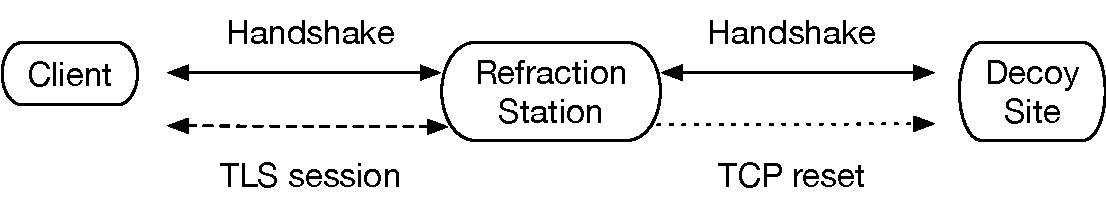
\includegraphics[width=\columnwidth]{figures/refraction-v1}
    \caption{First generation refraction networking designs operated as an inline transparent proxy.}
    \label{fig:refraction-v1}
\end{figure}

\begin{figure}
    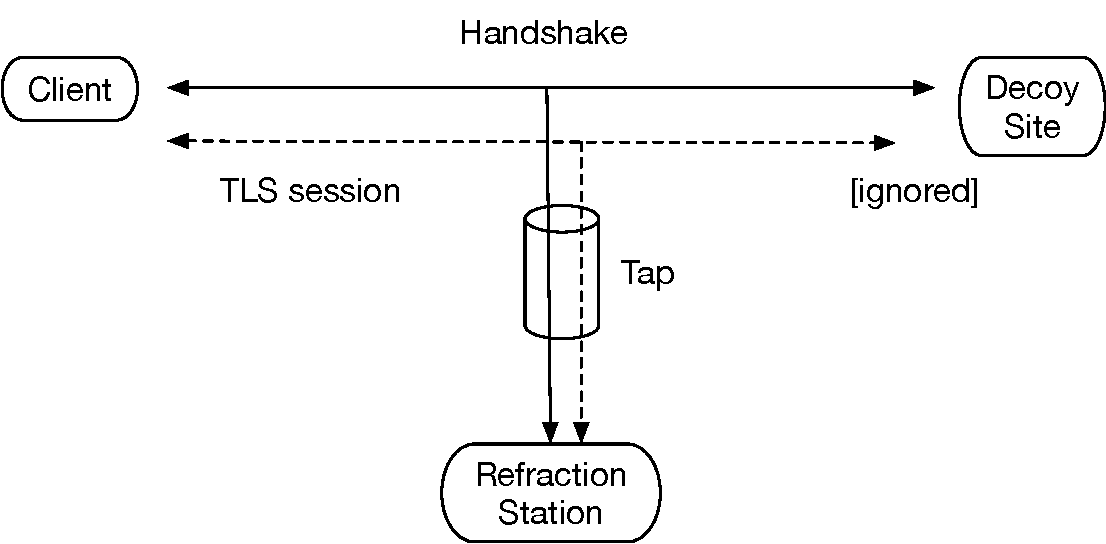
\includegraphics[width=\columnwidth]{figures/tapdance}
    \caption{TapDance operates without flow blocking by using a mirror
    port to receive a copy of traffic.}
    \label{fig:tapdance}
  \end{figure}

  \begin{figure}
    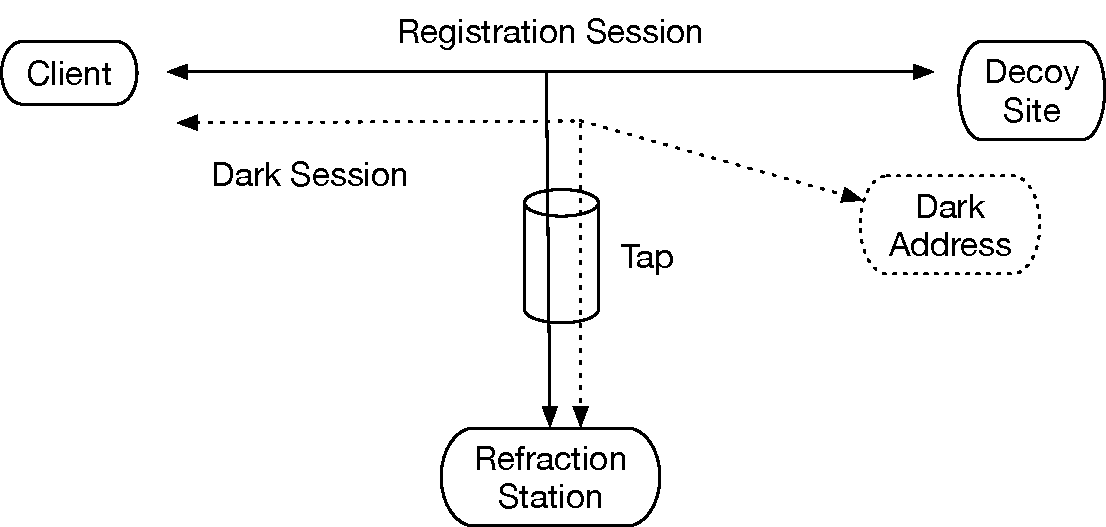
\includegraphics[width=\columnwidth]{figures/dark-decoys}
    \caption{Dark decoys uses two sessions: a registration one which is passively observed by the refraction station, and a dark session which is proxied by the RS in its entirety.}
    \label{fig:dark-decoys}
\end{figure}

One of the key challenges for refraction networking is in taking over a session. The RS must start responding to the client's traffic as if it were the decoy destination, and at the same time prevent the destination from sending its own responses back to the client. A simple approach is to have the refraction station act as an inline transparent proxy (\cref{fig:refraction-v1}) that forwards the traffic between the client and the decoy site. After a TLS handshake has been completed, the RS terminates the connection with the decoy site by sending a TCP reset and takes over the session with the client.

An inline element, however, can significantly affect the reliability and performance of the regular, non-refraction traffic of an ISP. Cirripede~\cite{cirripede} and Telex~\cite{telex} attempted to mitigate this by dynamically adding router rules to forward only a subset of traffic from a registered client or an active session through the element, but this nevertheless presented a deployability challenge.

TapDance~\cite{tapdance} offered an alternative design that did not require the blocking or redirection of traffic, but used a mirror port instead (\cref{fig:tapdance}). In TapDance a client sends an incomplete HTTP request, which causes the decoy site to pause waiting for more data while the RS takes over the connection in its place. After a client would receive a packet initiated by the RS, its TCP sequence numbers would become desynchronized with the decoy site, causing the decoy to ignore the packets sent by the client.

This approach reduced the barriers to deployment and TapDance was used in production during a pilot study, serving upwards of 50\,000 real-world users~\cite{tapdance-foci17}. \nikita{worth mentioning that it's being used in production again? we don't have a public ref for that though.} The tap-based approach, however, has some disadvantages. A decoy site will only ignore packets as long as the sequence numbers stay within its TCP window, and will terminate the connection after a timeout. Frolov et al.\ report that in their pilot, they eliminated roughly a third of potential decoy sites due to their measured window or timeout values being too small~\cite{tapdance-foci17}. Even so, sessions that try to upload non-trivial data amounts (in excess of about 15\,KB) or last longer than the timeout value (ranging from 30--120\,s) require the user to create new refraction connections, adding overhead, complexity, and opportunities for errors. Additionally, keeping the connections to the decoy site open for tens of seconds uses up the site's resources; Frolov et al.\ found that a default configuration of the Apache web server would only keep 150 simultaneous connections open, while pilot deployment would often result in dozens of connections to the same decoy site, creating a scaling concern.

Dark decoys are able to avoid these problems by splitting up the traffic between a registration session and a dark session \nikita{are these good terms?} (\cref{fig:dark-decoys}). The registration session is used to send a signal to the RS to let RS know that the client plans to use dark sessions and to establish a seed to be used in future communications (\cref{XXX}); the RS only passively observes this connection without any interference. The dark session connects to a dark address that is not routed to any host; the RS instead acts as a remote endpoint for the entirety of the connection, starting with the TCP handshake. This design obviates the need for taking over a session already in progress, which both simplifies the implementation and eliminates certain attacks, as we will discuss in \cref{XXX}.

\paragraph{Registration Signal} In all implementations of refraction networking, a client must send a covert signal to the RS to initiate communication. This covert signal is  embedded inside communication fields that must be indistinguishable from random by a censor without access to a secret/private key available to the station. Past implementations have used TCP initial sequence numbers~\cite{cirripede}, the ClientRandom field inside a TLS handshake~\cite{decoy-routing,telex}, and the encrypted body of an HTTPS request~\cite{tapdance}. In principle dark decoys can use any of these mechanisms for registration, but n our prototype we used the HTTPS request body as it offers the greatest flexibiity for the amount of data that can be sent with the registration.
